\documentclass[12pt]{article}
\usepackage{amsmath}
%\usepackage{mathtext}
\usepackage[french]{babel}
\usepackage{amsthm}
\usepackage{arydshln}
\usepackage{nccrules}

\usepackage{amsfonts}
\usepackage{amssymb}
\usepackage{latexsym}
\usepackage{eufrak}
\usepackage{tocloft}
\usepackage[center]{titlesec}
\usepackage[utf8]{inputenc}

%Для рисунков
\usepackage{graphicx}
\usepackage{graphics}
\usepackage{float}
\usepackage{caption}
\usepackage{topcapt}

%\usepackage{citesort}

%%%%%%%%%%%%%%%%%% DEFINE NEW COUNTERS %%%%%%%%%%%%%%%%%%%%%%%%%%%%%
\newcounter{isElectronicVersion} % Must be set as 1 if the electronic version with animations is to be created, otherwise the printed version will be created

%%%%%%%%%%%%%%%%%% SET NEW COUNTERS %%%%%%%%%%%%%%%%%%%%%%%%%%%%%
\setcounter{isElectronicVersion}{0} % 1 - electronic, 0 - printed

%%%%%%%%%%%%%%%%%% MATH OPERATORS %%%%%%%%%%%%%%%%%%%%%%%%%%%%%
\DeclareMathOperator\dv{div} % divegence
\DeclareMathOperator\id{I}   % identity matrix
\DeclareMathOperator\tr{tr}   % trace operator
\DeclareMathOperator\sgn{sgn}   % signum operator
%%%%%%%%%%%%%%%%%% BOLD SYMBOLS %%%%%%%%%%%%%%%%%%%%%%%%%%%%%
\newcommand{\bu}{\mathbf{u}}  % bold u
\newcommand{\bV}{\mathbf{V}}  % bold V
\newcommand{\bU}{\mathbf{U}}  % bold U
\newcommand{\bt}{\mathbf{t}}  % bold t
\newcommand{\bq}{\mathbf{q}}  % bold q
\newcommand{\bx}{\mathbf{x}}  % bold x
\newcommand{\be}{\mathbf{e}}  % bold e
\newcommand{\bbs}{\mathbf{s}}  % bold n
\newcommand{\bn}{\mathbf{n}}  % bold n
\newcommand{\bp}{\mathbf{p}}  % bold p
\newcommand{\bc}{\mathbf{c}}  % bold c
\newcommand{\bs}{\mathbf{s}}  % bold s
\newcommand{\cB}{{\cal B}} % calligraphic B
\newcommand{\mx}{\mathrm{max}}  % roman max
\newcommand{\mn}{\mathrm{min}}  % roman min
\newcommand\norm[1]{\left\lVert#1\right\rVert}
\newcommand{\bcu}{\mathbf{U}} % bold U
\newcommand{\bct}{\mathbf{T}} % bold T
\newcommand{\bpsi}{\bm{\psi}} % bold psi
\newcommand{\bsigma}{\bm{\sigma}} % bold sigma
\newcommand{\btau}{\bm{\tau}} % bold tau
%%%%%%%%%%%%%%%%%% CALLIGRAPHIC SYMBOLS %%%%%%%%%%%%%%%%%%%%%%%%%%%%%
\newcommand{\epss}{{\cal E}}
\newcommand{\cL}{{\cal L}}
\newcommand{\cT}{{\cal T}}
\newcommand{\cQ}{{\cal Q}}

%%%%%%%%%%%%%%%%%% DIFFERENTIAL OPERATORS %%%%%%%%%%%%%%%%%%%%%%%%%%%%%
\newcommand{\pd}[2]{ % partial first derivative
	\dfrac{\partial #1}{\partial #2}
} 
\newcommand{\opd}[2]{ % ordinary first derivative
	\dfrac{\mathrm{d} #1}{\mathrm{d} #2}
}
\newcommand{\pddB}[2]{ % partial first derivative with function bordered by braces
	\dfrac{\partial }{\partial #2}\Bigl(#1\Bigr)
} 
\newcommand{\pdd}[3]{ % partial second derivative
	\dfrac{\partial^2 #1}{\partial #2 \partial #3}
} 
%%%%%%%%%%%%%%%%%% NORM OPERATORS %%%%%%%%%%%%%%%%%%%%%%%%%%%%%
\newcommand{\normInf}[1]{|#1|_\infty} % infinity-norm

\newtheorem{dfn}{Definition}

\graphicspath{{img/}}

%Точечки в Содержании
\renewcommand{\cftsecleader}{\cftdotfill{\cftdotsep}}

%Центрирование Содержания
\renewcommand\cfttoctitlefont{\hfill\Large\bfseries}
\renewcommand\cftaftertoctitle{\hfill\mbox{}}

%Точка после Разделов в Содержании
\let \savenumberline \numberline
\def \numberline#1{\savenumberline{#1.}}

\begin{document}	
	\tableofcontents
	%\title{Influence of inhomogeneity of reservoir to the development of a hydraulic fracture in poroelastic medium}
	\title{Sofya Sizova, Anastasiya Dulepova}
	\maketitle
	\section{Énoncé du problème}
	On s'intéresse au problème 
	\begin{eqnarray} 
	\nonumber
	& &\text{Trouver } u \in C^2(0, T; L^2(\Omega)) \text{ telle que}\\[2mm]
	& &\begin{cases} \label{Initial_problem}
	\dfrac{\partial^2u}{\partial t^2} - \text{div} (\sigma\nabla u) = f \quad  \text{dans } \Omega \times [0, T_\text{max}]\\
	u|_{t = 0} = u_0 \quad \text{dans } \Omega \\
	\pd{u}{t}|_{t = 0} = u_1 \quad \text{dans } \Omega \\
	\sigma \pd{u}{n} = 0 \quad \text{sur } \partial\Omega \times [0, T_\text{max}]
	\end{cases}
	\end{eqnarray}
	Le coefficient $\sigma$ est supposé constant, avec une vitesse $c = 2$ et $\sigma = c^2$. 
	En multipliant l'équation \eqref{Initial_problem} par la fonction test $v \in H^1(\Omega)$ et un intégrant sur la domaine de $\Omega$, on obtiens la formulation variationnelle en utilisant les formules de Green. Il faut noter que si la solution forte $u$ de \eqref{Initial_problem} vérifie $u \in C^2(0, T; L^2(\Omega))$, on peut relaxer la régularité de solution en temps et utiliser le fait que
	\begin{equation*}
	\int_\Omega{\dfrac{\partial^2u}{\partial t^2}(x,t) v(x)d\Omega} = \frac{d^2}{dt^2} \int_\Omega{u(x,t) v(x)},
	\end{equation*}
	car la partie droite est bien définie au sens de distribution en raison de régularité suffisante. Donc, on suppose maintenant que $u \in C^1(0, T; L^2(\Omega))$ simplement. Il faut que la fonction $u$ soit $C^1$ minimum, car les conditions initiales doivent pouvoir être définies ponctuellement.  Alors, la formulation variationnelle est la suivante
	\begin{eqnarray}
	\nonumber
	& &\text{Trouver u} \in C^1(0, T; L^2(\Omega)) \cap C^0(0, T; H^1(\Omega)) \text { tel que}\\
	& &\begin{cases} \nonumber
	\dfrac{d^2}{dt^2} \int_\Omega {u v d\Omega} + \int_\Omega{\sigma \nabla u \nabla v d\Omega} = \int_\Omega{f v d\Omega} \quad \forall v \in H^1(\Omega) \text{ p.p } t \in (0,T),\\
	u(x, 0) = u_0, \quad \pd{u}{t}(x,0) = u_1 \quad \text{dans } \Omega \\
	\sigma \pd{u}{n} = 0, \text{sur } \partial\Omega \times [0, T_\text{max}]
	\end{cases}
	\end{eqnarray}
	
	
	Pour obtenir l'identité d'énergie on multiple la première équation de   \eqref{Initial_problem} par $\pd{u}{t}$ et intègre sur $\Omega$. Donc
	\begin{equation}
	\label{energie1}
	\int_\Omega{\dfrac{\partial^2u}{\partial t^2} \pd{u}{t} d\Omega} - \int_\Omega{\text{div}(\sigma \nabla u)\pd{u}{t} d\Omega} = \int_\Omega{f \pd{u}{t} d\Omega}.
	\end{equation}
	On peut modifier le première terme de \eqref{energie1} comme
	\begin{equation*}
	\int_\Omega{\dfrac{\partial^2u}{\partial t^2} \pd{u}{t} d\Omega}= \frac{1}{2}\int_\Omega{\frac{d}{dt}(\pd{u}{t})^2d\Omega} = \frac{1}{2}\frac{d}{dt}\int_\Omega{(\pd{u}{t})^2d\Omega} = \frac{1}{2}\frac{d}{dt}\|\pd{u}{t}\|^2_{L^2(\Omega)}.
	\end{equation*}
	La deuxième égalité est admissible car la régularité de $u$ est suffisante selon les hypothèses ci-dessus.
	Le second terme de \eqref{energie1} est égal à $\int_\Omega{\sigma \nabla u \nabla(\pd{u}{t}) d\Omega}$ par la formule de Green et la condition au bord de $\Omega$ pour $\pd{u}{n}$. Donc, on peut s'amener à
	\begin{multline*}
	\int_\Omega{\sigma \nabla u \nabla(\pd{u}{t}) d\Omega} = \int_\Omega{\sigma \nabla u\pd{\nabla u}{t} d\Omega} = \int_{\Omega}{\frac{d}{dt}\frac{1}{2}(\sqrt{\sigma}\nabla u)^2} =\\ \frac{1}{2}\frac{d}{dt}\int_{\Omega}{(\sqrt{\sigma}\nabla u)^2} \text{ par hypothèses de régularité }
	= \frac{1}{2}\frac{d}{dt}\|\sqrt{\sigma}\nabla u\|^2_{L^2(\Omega)}.
	\end{multline*}
	Donc, l'énergie est définie par $E(t) = \dfrac{1}{2}\|\pd{u}{t}\|^2_{L^2(\Omega)} + \dfrac{1}{2}\|\sqrt{\sigma}\nabla u\|^2_{L^2(\Omega)}$, et on a l'identité
	\begin{equation*}
	\dfrac{d E(t)}{dt} = (f(t),\pd{u}{t})_{L^2(\Omega)},
	\end{equation*}
	Si $f = 0$, alors $E = E_0 = \frac{1}{2}\|u_1\|^2 + \frac{1}{2}\|\sqrt{\sigma}\nabla u_0\|^2$, i.e. l'énergie se conserve en l'absence de source.
	\section{Discrétisation}
	Maintenant on discrétise cette formulation variationnelle par les éléments finis de Lagrange $P^1$ en espace et différences finies centrées d’ordre 2 en temps. On va tout d'abord discrétiser l'espace en utilisant le méthode de Galerkin. Soit $V_h$ est de dimension fini et $V_h \subset H^1(\Omega)$, qui vérifie la propriété d'approximation, c'est à dire quand $h$ tend vers 0, $\underset{v_h\in V_h}{\inf}\|v - v_h\|$ tend vers zéro $\forall v \in H^1(\Omega)$. Alors, la formulation variationnelle semi-discrète est
	\begin{eqnarray}
	\nonumber
	& &\text{Trouver } u_h \in C^1(0, T; V_h) \text{ tel que}\\[2mm]
	\label{semi-discrete}
	& &\begin{cases}
	\dfrac{d^2}{dt^2} \int_\Omega {u_h v_h d\Omega} + \int_\Omega{\sigma \nabla u_h \nabla v_h d\Omega} = \int_\Omega{f v_h d\Omega} \quad \forall v_h \in V_h \text{ p.p } t \in (0,T),\\
	u_h(0) = u_{h,0}, \quad \frac{d u_h}{dt}(0) = u_{h,1} \quad \text{dans } \Omega \\
	\sigma \pd{u}{n} = 0, \text{sur } \partial\Omega \times [0, T_\text{max}]
	\end{cases}
	\end{eqnarray}
	On introduit la base de $V_h$ $(\omega_i)_{i = 1..N}$, où $N = \dim{V_h}$. Donc, on peut écrire $u_h$
	\begin{equation*}
	u_h(t) = \sum_{i = 1..N}{u_h(M_i, t)\omega_i} = \sum_{i = 1..N}{U_i(t)\omega_i}.
	\end{equation*} 
	Alors, on peut réécrire la formulation \eqref{semi-discrete} dans une forme matricielle
	\begin{eqnarray}
	\begin{cases} \label{matr_semi_discrete}
	\mathbb{M}\frac{d^2U}{dt^2}(t) + \mathbb{K}^\sigma U(t) = F(t)\\
	U(0) = U_0, \quad \frac{dU}{dt}(0) = U_1,
	\end{cases}
	\end{eqnarray}
	où $\mathbb{M}_{ij} = \int_\Omega{\omega_i \omega_j d\Omega}$, $\mathbb{K}_{ij}^\sigma = \int_\Omega{\sigma\nabla\omega_i \nabla\omega_j d\Omega}$ sont les matrices symétriques, positives (car $(\mathbb{M}V,V) = \|v_h\|^2 > 0$, et $(\mathbb{K}V,V) = \|\sigma\nabla v_h\|^2 > 0$) et en plus définies positives (car $\omega_i \in H^1_0$ et dans cet espace on a l'inégalité de Poincaré), $F_j = \int_{\Omega}{f\omega_i d\Omega}$.
	
	
	Pour la discrétisation en temps on considère $U_i^k = U_i(t_k)$, donc\\ $u_h^k = \sum_{i = 1..N}U_i^k\omega_i$. On va discrétiser la seconde dérivative dans \eqref{semi-discrete} par le schéma d'ordre 2, le schéma saute-mouton. Donc, l'équation dans \eqref{matr_semi_discrete} discrétisé en temps est
	\begin{equation*}
	\mathbb{M}\dfrac{U^{k+1} - 2U^k + U^{k - 1}}{\Delta t^2} + \mathbb{K}^\sigma U^k = F^k.
	\end{equation*}
	Ici $\Delta t $ = $\frac{T}{M}$, $M$ es le nombre de couches en temps.
	Il faut définir les conditions initiales dans ce cas. En $t = 0$ on a $u_h(0) = u_h^0 \approx u_{h,0}$. Pour le prochain pas du temps $t_1 = \Delta t$ on utilise la formule de Taylor d’ordre 2
	\begin{equation*}
	u(\Delta t) = u_0 + \Delta t u_1 + \frac{\Delta t^2}{2}\frac{\partial^2u}{\partial t^2}(0) + O(\Delta t^3)
	\end{equation*}
	D'auprès l'équation initiale \eqref{Initial_problem} cela conduit (variationnellement) à l'approximation 
	\begin{multline*}
	(u_h(\Delta t), v_h)_{L^2} = (u_h^1, v_h)_{L^2} \approx (u_{h,0}, v_h)_{L^2} + \Delta t(u_{h,1},v_h)_{L^2} -\\ \frac{\Delta t^2}{2}(\sigma \nabla u_{h,0}, \nabla v_h)_{L^2} + \frac{\Delta t^2}{2} (f(0), v_h)_{L^2}
	\end{multline*}
	car $\dfrac{\partial^2u}{\partial t^2} = \sigma \Delta u + f$ dans notre cas homogène avec $\sigma = c^2 = const$.
	Alors à partir de Taylor on déduit la condition initiale matricielle
	\begin{equation*}
	\mathbb{M}U^1 = \mathbb{M}U_0 + \Delta t\mathbb{M}U_1 - \frac{\Delta t^2}{2}c^2\mathbb{K}U_0 +  \frac{\Delta t^2}{2}F^0.
	\end{equation*}
	L'indice supérieur signifie un pas de temps, et inférieur signifie le pas d'espace. Finalement, le schéma totalement discrétise est \eqref{total-discr}.
	\begin{eqnarray}
	\label{total-discr}
	\begin{cases}
	\mathbb{M}\dfrac{U^{k+1} - 2U^k + U^{k - 1}}{\Delta t^2} +\sigma \mathbb{K} U^k = F^k,\\
	U^0 = U_0,\\
	\mathbb{M}U^1 = \mathbb{M}U_0 + \Delta t\mathbb{M}U_1 - \frac{\Delta t^2}{2}\sigma \mathbb{K}U_0 +  \frac{\Delta t^2}{2}F^0.
	\end{cases}
	\end{eqnarray}
	On peut accélérer ce schéma en augmentant le pas de temps $\Delta t$ ou la taille de discrétisation en espace $h$. Mais il est important de se rappeler que les valeurs arbitraires de $h$ et $\Delta t$ peuvent entraîner une instabilité de schéma. Il faut que ces valeurs satisfassent l'inégalité de stabilité (la condition de Courant–Friedrichs–Levy), qui sera donnée ci-dessous. De plus, le schéma peut être accéléré si, au lieu d'utiliser la matrice de masse exacte, on utilisera la matrice de masse condensée, qui approche la matrice exacte et qui est diagonale et, par conséquent, son inverse est très facile à calculer.
	\section{L'identité d'énergie discrète}
	On définit une énergie discrète du schéma $\mathcal{E}$, qui représente l'approximation de l'énergie continue $E(t)$.
	\begin{equation*}
	\mathcal{E}^{k + 1/2} = \frac{1}{2}\norm{\frac{U^{k+1} - U^k}{\Delta t}}_\mathbb{M}^2 + \frac{1}{2}(c^2\mathbb{K}U^k, U^{k+1}).
	\end{equation*}
	Ici $\norm{U}_\mathbb{M}^2 = (\mathbb{M}U,U)$. Pour obtenir l'inégalité d'énergie discrète on multiple la première équation de \eqref{total-discr} par $\frac{U^{k+1} - U^{k - 1}}{2\Delta t}$. En regroupant les termes, nous obtenons
	\begin{multline*}
	\frac{1}{2}\mathbb{M}\frac{(U^{k+1} - U^k)^2 - (U^k - U^{k-1})^2}{\Delta t^2} + \frac{1}{2}(c^2\mathbb{K}U^k, U^{k+1}) - \frac{1}{2}(c^2\mathbb{K}U^{k}, U^{k-1}) \\= \Delta t(F^k, \frac{U^{k+1} - U^{k - 1}}{2\Delta t}).
	\end{multline*}
	Donc on voit qu'en l'absence de source l'énergie discrète se conserve.
	\begin{equation}
	\label{energie-discrete}
	\mathcal{E}^{k +1/2} = \mathcal{E}^{k - 1/2} \quad \forall k \geq 1.
	\end{equation}
	Pour en déduire la condition de stabilité à partir d'égalité \eqref{energie-discrete}, il faut s'assurer que $(c^2\mathbb{K}U^k, U^{k+1})$ soit définie positive. Cela conduit à la formulation d'une condition de stabilité nécessaire de type CFL \eqref{CFL1}.
	\begin{equation}
	\label{CFL1}
	\gamma_{\text{cfl}} = \frac{c^2 \Delta t^2}{4}\sup_{V \neq 0} \frac{(\mathbb{K}V, V)}{(\mathbb{M}V, V)} \leq 1.
	\end{equation}
	On peut utilisé la théorie connue pour exprimer cette condition dans une autre forme.
	\begin{eqnarray}\nonumber
	& &\gamma_{\text{cfl}} = \frac{c^2 \Delta t^2}{4} \sup_i|\lambda_i|, \text{où}\\
	\nonumber
	& &\lambda_i \text{ sont les solution de probleme aux valeurs propres}\\
	\label{propres}
	& &\begin{cases}
	-\text{div}(\sigma\nabla u ) = \lambda u,\\
	\sigma \pd{u}{n} = 0 \quad \text{sur } \partial\Omega
	\end{cases} \\
	\nonumber
	& &\text{ qui est equivalente de la formulation matricielle } c^2\mathbb{K}U = \lambda_h \mathbb{M}U.
	\end{eqnarray}
	Alors, le schéma est stable, si le pas en temps 
	\begin{equation}
	\label{CFL}
	\Delta t \leq \frac{2}{c \sqrt{\sup |\lambda_i|}}.
	\end{equation}
	Pour donner l'expression plus précise il faut calculer le spectre du problème \eqref{propres}.
	
	\section{Condensation de masse}
	L'inconvénient de la formulation \eqref{total-discr} est que le schéma n'est pas explicite et on doit chaque fois inverser la matrice $\mathbb{M}$. On veut approcher la matrice de masse $\mathbb{M}$ par une matrice diagonale en utilisant les formules de quadratures suivante
	\begin{equation*}
	\int_{\mathcal{T}}{g(x) dT} \approx \frac{|\mathcal{T}|}{3}\sum_{i = 1}^3{g(S_i)},
	\end{equation*}
	où $\mathcal{T}$ est une triangle dans le maillage avec l'aire égal à $|\mathcal{T}|$ et $S_i, i = 1,2,3$ sont ses sommets.
	Dans notre cas $g(x)$ est $w_\alpha(x)w_\beta(x)$ ($w$ sont les fonctions de base) et pour la matrice de masse élémentaire approchée on a 
	\begin{equation*}
	\mathbb{M}^{elem, ap}_{\alpha \beta} \approx \frac{|\mathcal{T}|}{3}\sum_{i=1}^{3} {w_\alpha(S_i) w_\beta(S_i)} = \frac{|\mathcal{T}|}{3} \delta_{\alpha \beta}.
	\end{equation*}
	Pour calculer la matrice condensée on somme les matrices élémentaires sur tout les triangles. Et on obtient alors une matrice diagonale $\mathbb{M}^{cond}$.
	
	Les expressions pour la matrice de rigidité et la matrice de masse sans condensation sont présentées ci-dessus.
	\section{Le pas de temps autorise par la condition de CFL}
	En résolvant le problème \eqref{propres} numériquement pour le maillage comme dans fig. \ref{fig:maillage1} on a trouvé les plus grandes valeurs propre $\lambda^{sup}_h$ pour $h = 0.02j, j = 1..10$. Donc, par \eqref{CFL} on obtiens l'estimations pour $\Delta t$, qui sont présentés dans le tableaux dessous.
	\begin{figure}[h]
		\centering
		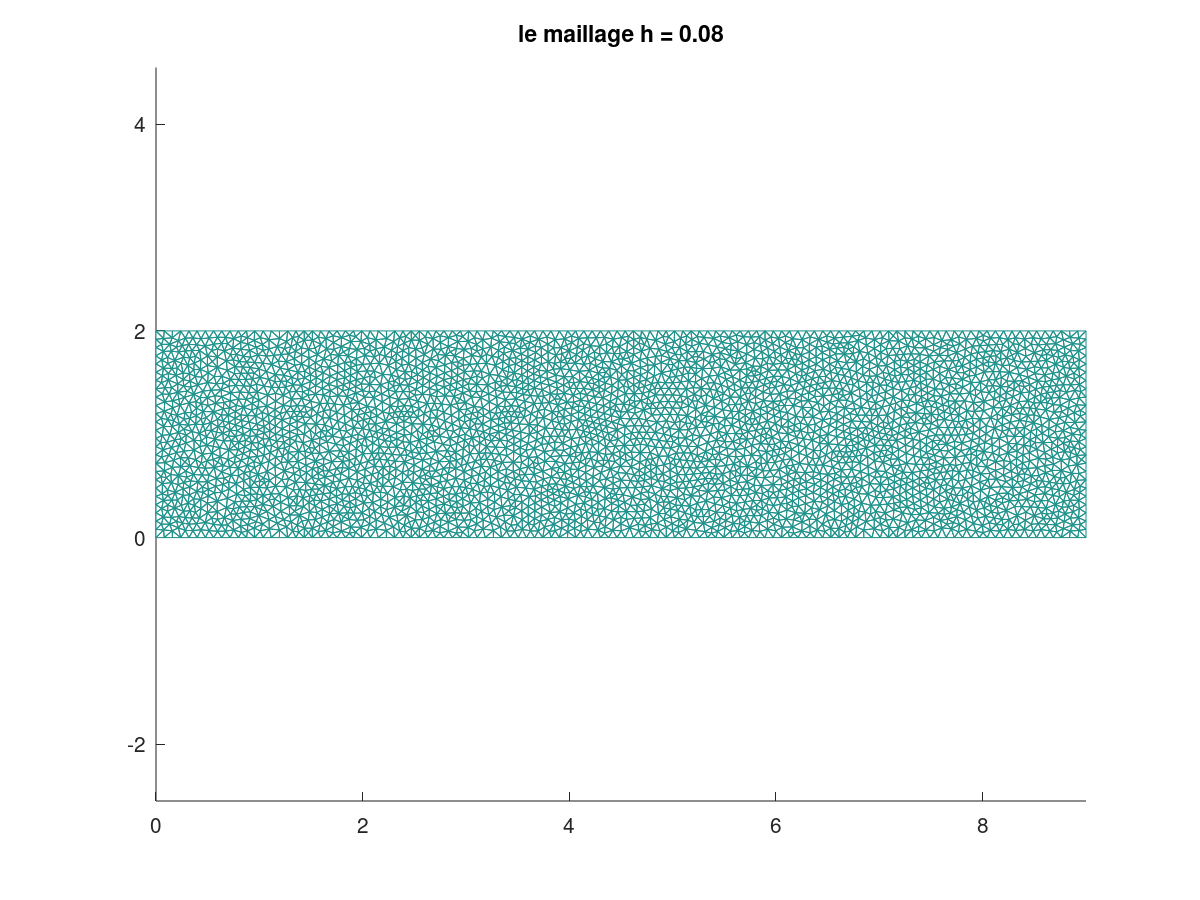
\includegraphics[height=0.4\linewidth]{images/maillage1}
		\caption{La discrétisation de domaine  avec $h = 0.8$.}
		\label{fig:maillage1}
	\end{figure}
	\begin{table}[H]
		\caption{\label{tab:canonsummary} Le pas de temps maximum autorisé par la condition CFL pour la matrice exacte (gauche) et la matrice condensée (droite) }
		\begin{center}
			\begin{tabular}{|c|c|c|}
				\hline
				$h$ & $\Delta t_{ex}$ & $\Delta t_{cond}$ \\
				\hline
				0.02 & 0.003 &  0.005 \\ 
				0.04 & 0.005 & 0.01 \\
				0.06 & 0.009 & 0.015\\
				0.08 & 0.012 & 0.021\\
				0.1  & 0.015 & 0.026\\
				0.12 & 0.018 & 0.031\\
				0.14 & 0.022 & 0.036\\
				0.16 & 0.024 & 0.04\\
				0.18 & 0.029 & 0.049\\
				0.2  & 0.028 & 0.052\\
				\hline
			\end{tabular}
		\end{center}
	\end{table} 
	On voit que les conditions CFL pour la matrice de masse condensée sont moins restrictives (on a $\Delta t$ plus grands) ce qui est un autre avantage de cette approche.
	\section{La partie droite}
	La partie droite dans \eqref{total-discr} est calculée à l'aide d'une méthode d'interpolation.
	
	Car
	\begin{equation*}
	f(t) \approx \sum_{J} f(t,M_J)w_J,
	\end{equation*}
	on peut approcher le second membre (qui a des composants $F^k_I = F_I(t_k) = \int_\Omega f(t_k) w_I d\Omega$) par
	\begin{equation*}
	F^k \approx M\tilde{F}^k \quad \text{avec} \quad \tilde{F}^k = f(t_k,M_J)_{J=1,N}.
	\end{equation*}
\section{Résultats de calcul}
Les figures ci-dessous montrent les solutions obtenues aux instants $T \approx 2$ et $T \approx 4$ (vue de dessus à la surface) pour le maillage avec $h=0.1$.
\begin{center}
	\hspace{1cm}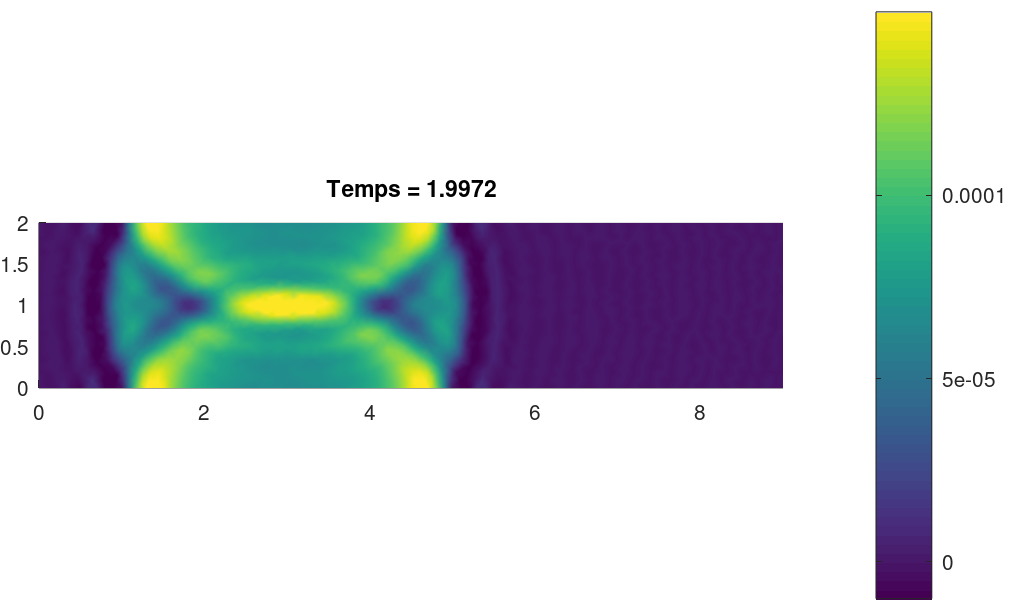
\includegraphics[width=0.4\textwidth]{images/T2.png}\hspace{1cm}
	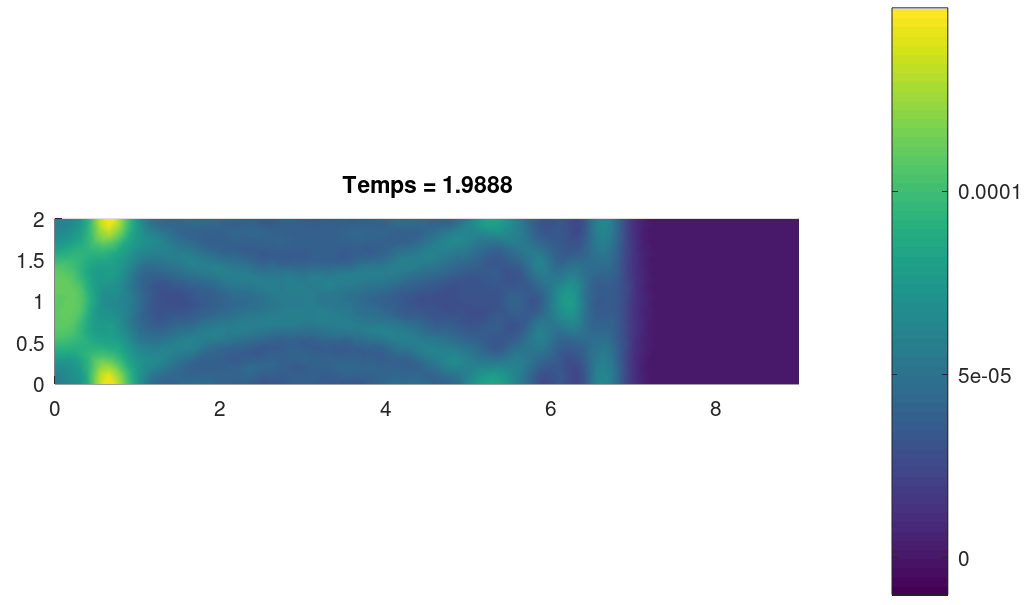
\includegraphics[width=0.4\textwidth]{images/T2condense.png}\hspace{1cm}
	{La distribution de solution pour $T \approx 2$ pour la matrice exacte (à gauche) et matrice condensée (à droite)}.
\end{center}

\begin{center}
	\hspace{1cm}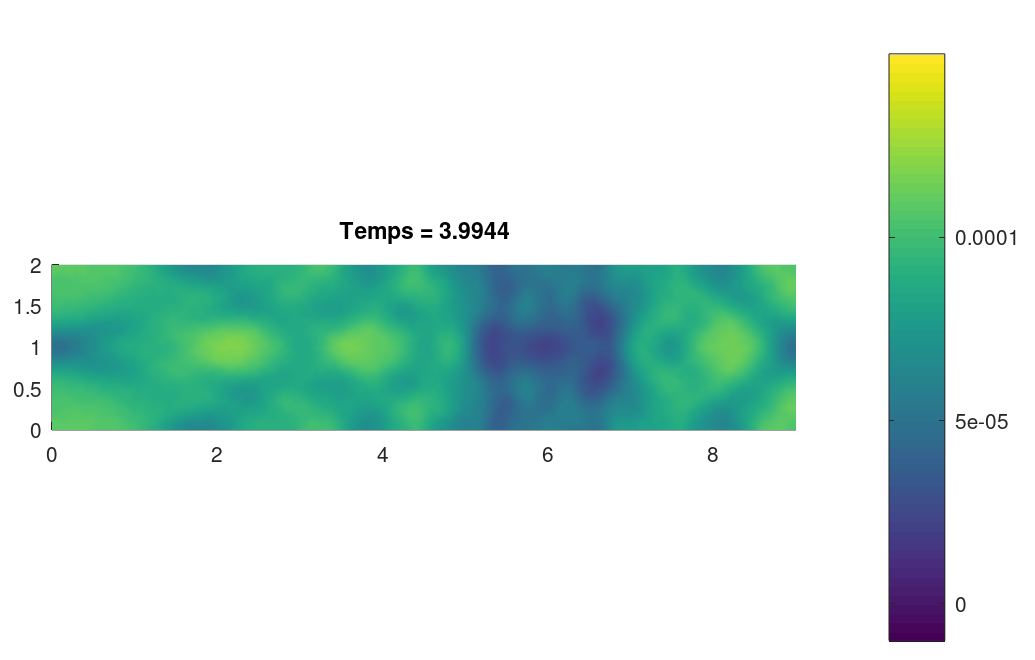
\includegraphics[width=0.4\textwidth]{images/T4.png}\hspace{1cm}
	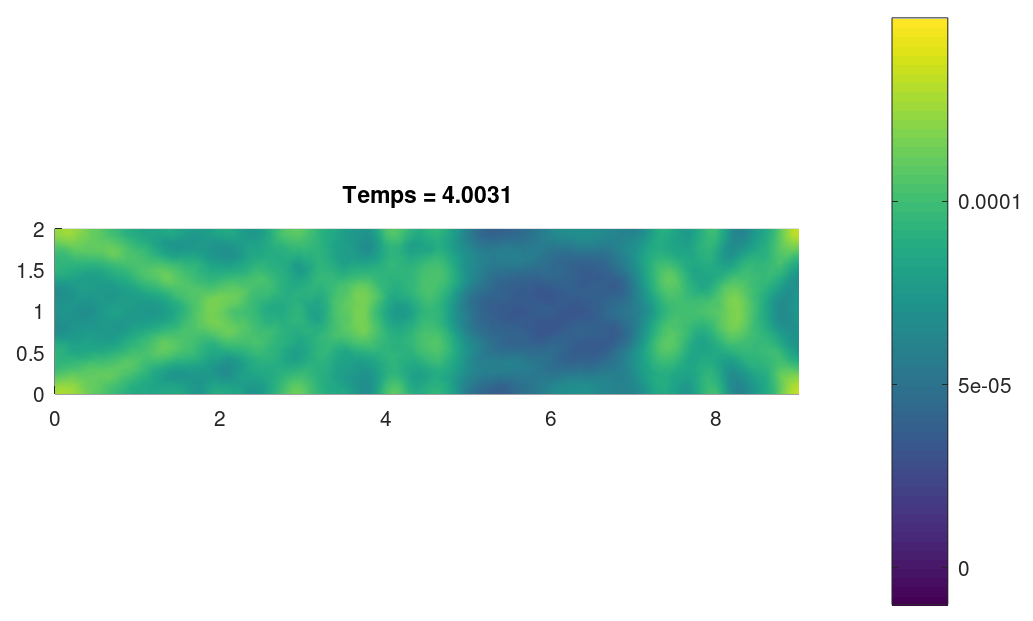
\includegraphics[width=0.4\textwidth]{images/T4cond.png}\hspace{1cm}
	{La distribution de solution pour $T \approx 4$ pour la matrice exacte (à gauche) et matrice condensée (à droite)}.
\end{center}
\section{L'énergie discrète}
L'évolution d'énergie discrète est affichée dans la fig. \eqref{fig:energie_e} pour la matrice de masse exacte et  pour la matrice de masse condensée dans la fig. \eqref{fig:energie_c}. On peut voir que  au début l'énergie est nulle (car les conditions initiales sont nulles), mais à partir de certain temps $t_0 \approx 0.1$ l'énergie est égale à une constante très petite. Cela correspond bien à la théorie, parce que pour $t$ assez grande la partie droite $f(x, y, t) = e^{-50(t + 0.2)^2 e^{-50((x - 3)^2 + (y - 1)^2)}} $ devient assez petite. Et on sait bien, que en l'absence de source l'énergie discrète se conserve.
\begin{figure}[H]
	\centering
	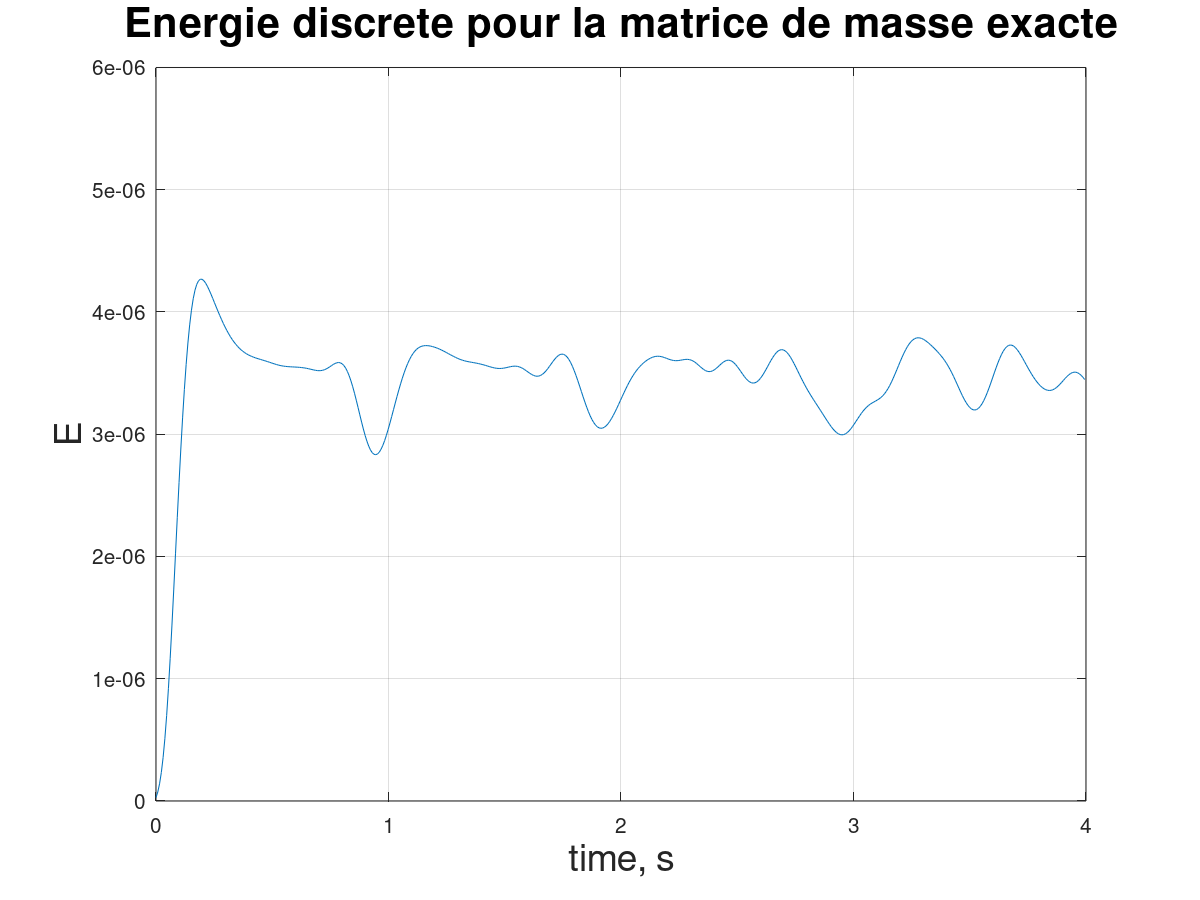
\includegraphics[height=0.4\linewidth]{images/E_01}
	\caption{L'énergie discrète pour la matrice de masse exacte, $h=0.1$.}
	\label{fig:energie_e}
\end{figure}
\begin{figure}[H]
	\centering
	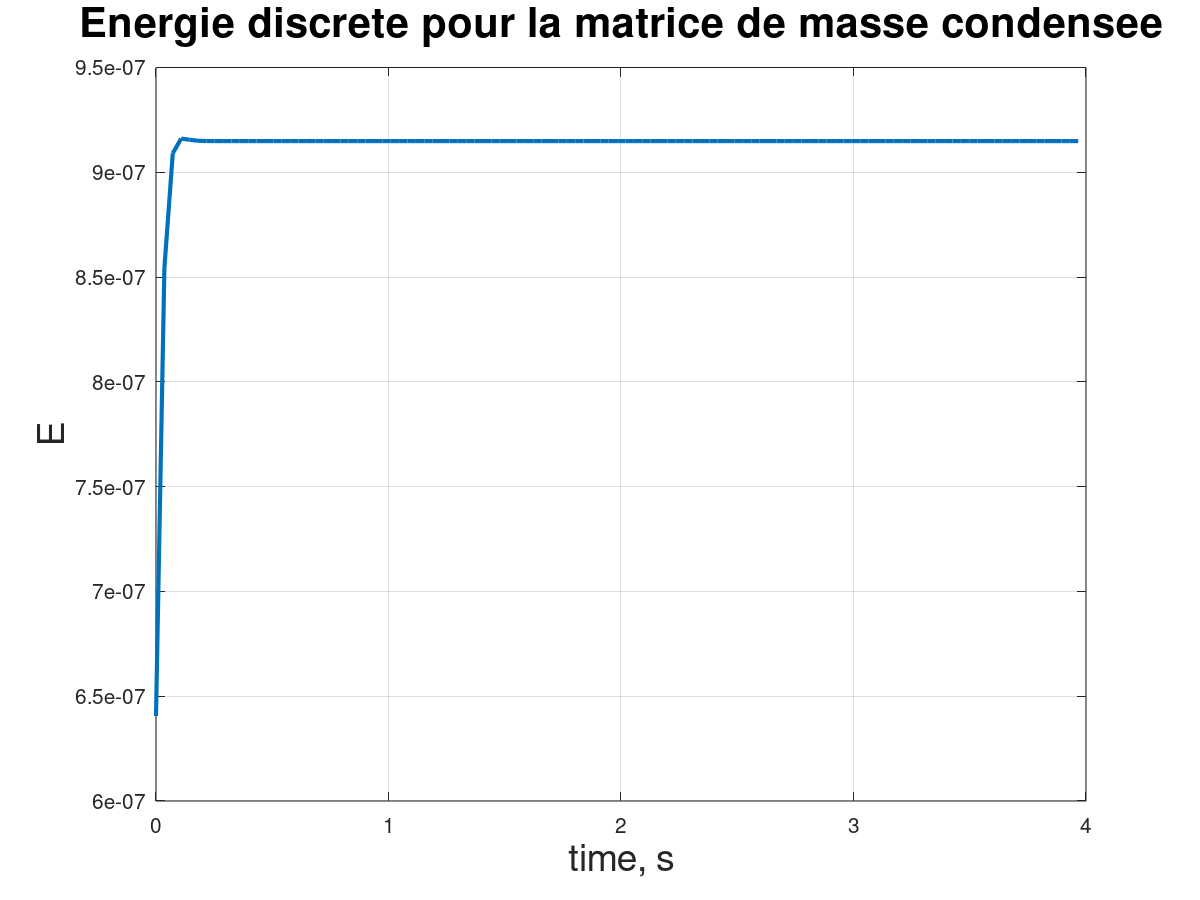
\includegraphics[height=0.4\linewidth]{images/E_cond_01}
	\caption{L'énergie discrète pour la matrice de masse condensée, $h=0.1$.}
	\label{fig:energie_c}
\end{figure}	

\section{L'évolution de la solution au point}
Les figures \eqref{fig:u_point_exacte} et \eqref{fig:u_point_cond} représentent l'évolution de la solution numerique au point le plus proche de $(6.5,1)$ de maillage (le maillage avec $h=0.1$). Fig.\eqref{fig:u_point_exacte} correspond au cas de matrice de masse exacte et fig.\eqref{fig:u_point_cond} au cas de matrice condensée.
\begin{figure}[H]
	\centering
	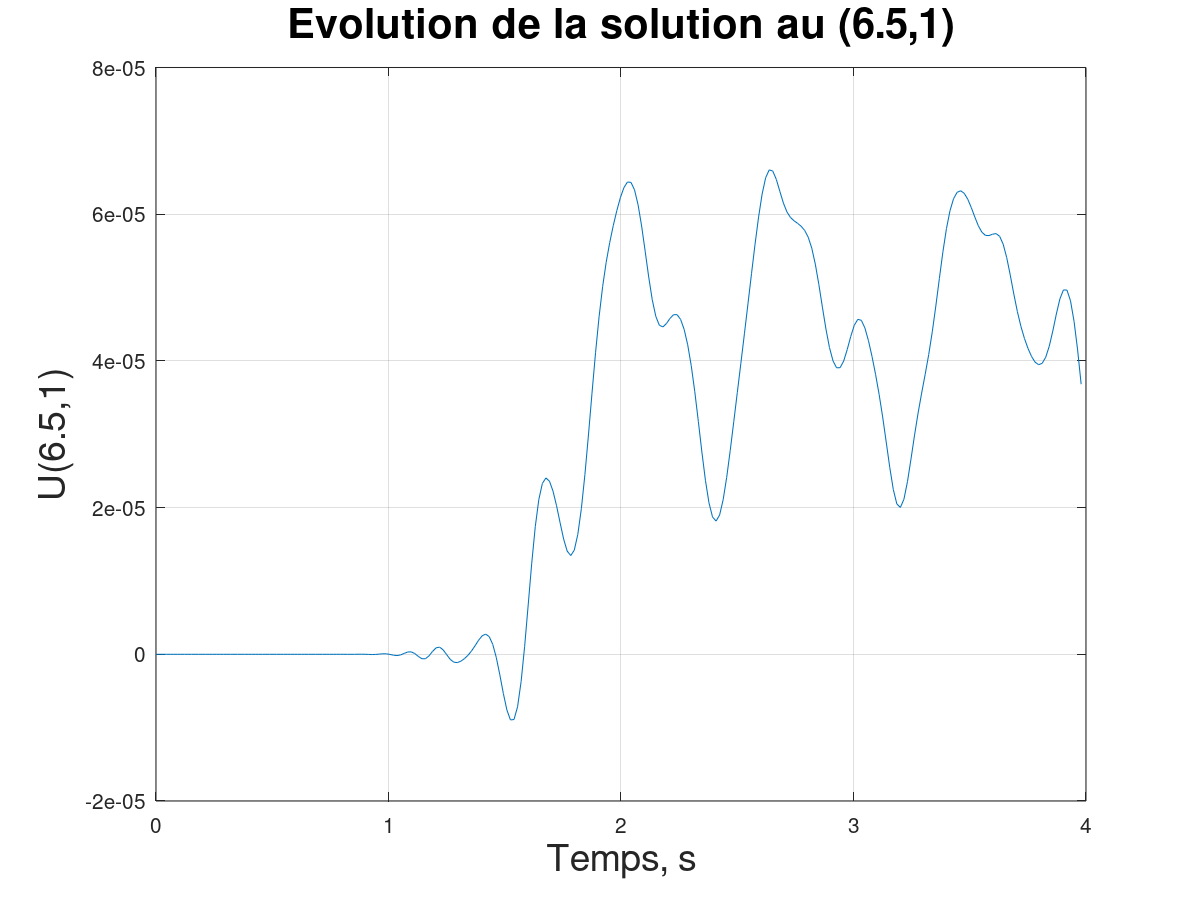
\includegraphics[height=0.4\linewidth]{images/u_6,5,1}
	\caption{L'évolution de la solution au (6.5,1), la matrice de masse exacte.}
	\label{fig:u_point_exacte}
\end{figure}
\begin{figure}[H]
	\centering
	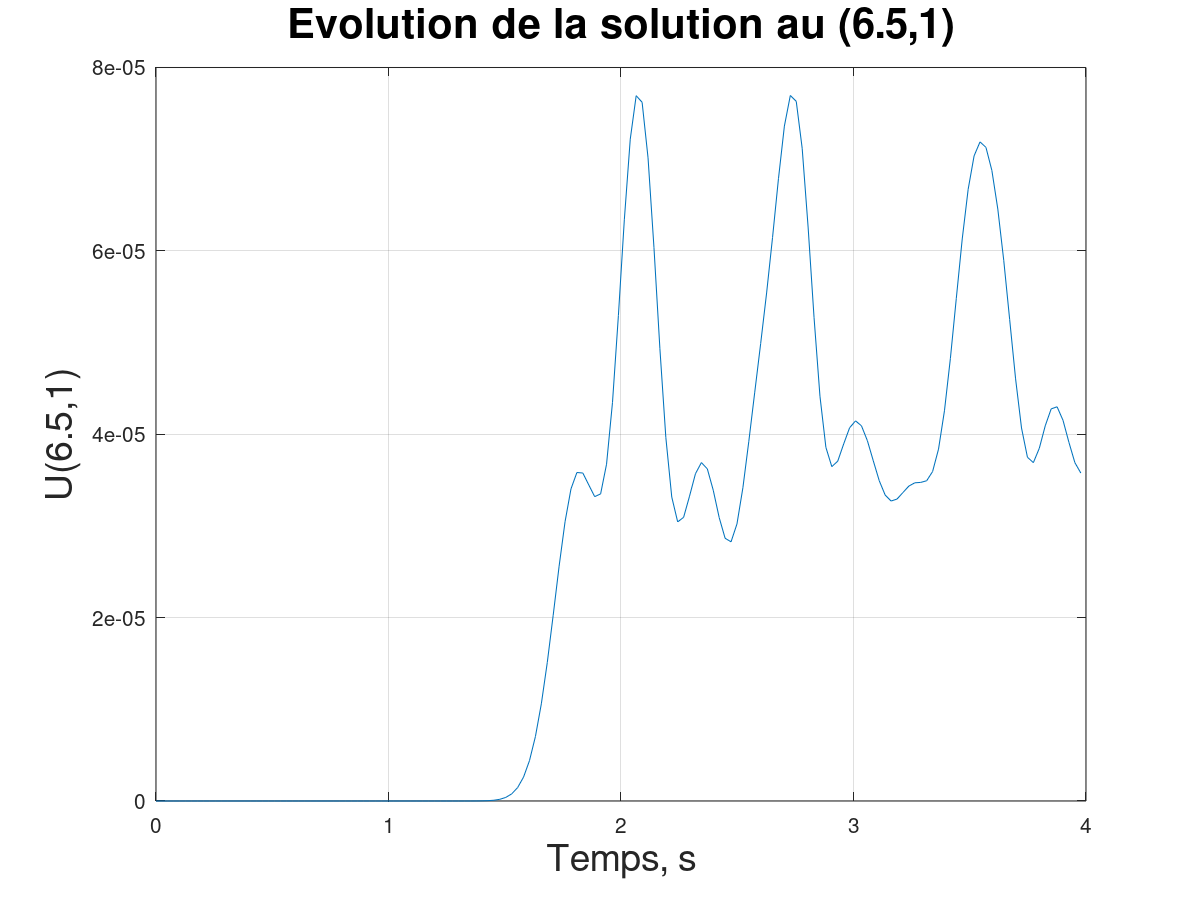
\includegraphics[height=0.4\linewidth]{images/u_6,5,1_condense}
	\caption{L'évolution de la solution au (6.5,1), la matrice de masse condensée.}
	\label{fig:u_point_cond}
\end{figure}
On peut remarquer que dans les deux cas, jusqu'à un certain point dans le temps, la solution est nulle, puis elle change, ce qui correspond au moment où l'onde atteint ce point. Pour la matrice de masse exacte ce moment est égal à environ 1 seconde (mais les oscillations plus significatives viennent à $\approx 1.5 s$), et pour la matrice condensée environ 1.5 secondes. La différence entre les solutions est moins que $2\cdot10^{-6}$, ce qui est bien précis pour le maillage avec $h=0.1$. 

\section{Le temps de calcul}
Les temps de calcul pour la matrice de masse exacte sont les suivants (on considère le maillage avec $h=0.1$ et on exécute le programme en Octave):
\begin{itemize} 
	\item  347.77s avec affichage de la solution à chaque pas de temps
	\item  3.77s sans affichage.
\end{itemize}
Pour la matrice condensée:
\begin{itemize} 
	\item  210.2s avec affichage de la solution à chaque pas de temps
	\item  0.14s sans affichage.
\end{itemize}
A partir de ces chiffres (notamment des temps de calcul sans affichage, car l'affichage prend beaucoup de temps), il est évident que le schéma avec la matrice de masse condensée est beaucoup moins coûteaux que celui avec la matrice exacte (environ 27 fois plus rapide sans affichage). Pour le maillage avec $h=0.08$, par exemple, on a le temps de calcul sans affichage pour $\mathbb{M}^{exacte}$ égal à 12.05s et pour $\mathbb{M}^{cond}$ égal à 0.17s, ce qui est encore mieux ($\approx 71$ fois plus rapide).

\section{CFL}
Pour le maillage avec $h=0.1$ on a calculé $\Delta t$ à partir de formule \eqref{CFL} avec égalité. On a obtenu dans le cas de matrice de masse exacte $\Delta t_{calcul\acute{e}} = 0.015246$. Après la variation de pas de temps on a vu que jusqu'à $\Delta t = 0.0153$ il y a la stabilité de solution: la valeur absolue maximale (parmi les valeurs aux points du maillages) de la solution est toujours (c'est à dire, pour chaque instant $t$ jusqu'à $T=4$) inférieure à $10^{-3}$, mais après pour $\Delta t = 0.01531$ on a déjà la valeur absolue maximale égale à 9.5921 et après pour $\Delta t = 0.154$ ce maximum atteint $2.25 \cdot 10^{12}$, qui montre clairement l'instabilité.

Pour la matrice condensée ($h$ est toujours égal à 0.1) $\Delta t_{calcul\acute{e}} = 0.025498$. Pour $\Delta t = 0.0263$ on voit déjà la croissance de la valeur absolue maximale de la solution jusqu'à 357.2. Alors que avant $\Delta t = 0.026$ c'est toujours inférieure à $10^{-3}$. Pour $\Delta t = 0.027$ la solution explose jusqu'à $5.6 \cdot 10^{10}$. Autrement dit, l'instabilité aussi.

Ainsi, on conclut que la CFL numerique correspond (i.e. qu'elle coïncide avec une grande précision) à celle prédite par la théorie (l'expression \eqref{CFL}).

\end{document}